
\section{Identity and Individuation}
\label{sec:identity-and-individuation}

\subsection{The Ontological Problem of Individuation}

The problem of individuation concerns how an existent is
constituted as a distinct existent. It addresses a question
that cannot be fully answered through the concepts of identity,
unity, or distinction considered independently.

Identity concerns the determinate character through which
an existent is the existent that it is. Unity concerns the
condition through which an existent constitutes a unity.
Distinction concerns the difference or non-identity between
existents or determinations. Individuation, however, concerns
the ontological constitution through which an existent is
determined as this distinct existent.

The problem is not merely how one entity can be distinguished
from another through description. It concerns the ontological
conditions under which an existent is an individual existent
rather than an undifferentiated possibility or an aspect
of something else.

Individuation must therefore be treated as an ontological
problem rather than exclusively as a logical, classificatory,
or epistemological operation.

The present analysis does not assume that individuation
is produced by a knowing subject, by the act of identifying
an entity, or by assigning a particular designation to it.
An existent is not constituted as an individual merely
because it is recognized or classified as one.

The task is to examine individuation as a condition
belonging to the ontological constitution of existents
themselves.

\subsection{Individuation and Identity}

Individuation and identity are closely related, but they
are not interchangeable.

Individuation concerns how an existent is constituted
as a distinct existent. Identity concerns what makes
that existent the existent that it is.

If individuation were identical to identity, the
ontological question of how an existent is constituted
as an individual would become indistinguishable from
the question of its determinate character.

Such a reduction would obscure an important distinction.
The constitution of an existent as an individual and
the constitution of its identity may be related aspects
of the same ontological actuality, but they do not
necessarily answer the same question.

An existent may be individuated, yet the complete
structure of its identity may remain to be investigated.
Likewise, an account of identity cannot be considered
complete merely because the existent has been
distinguished as an individual.

The relation between the two concepts must therefore
be established without reducing either to the other.

This distinction also prevents individuation from
being treated as a mere consequence of possessing
a distinctive descriptive profile. A description
may characterize an individual, but it does not
necessarily explain the ontological conditions
through which that individual exists as such.

\subsection{Individuation and Unity}

Individuation is also related to unity.

An individual existent may constitute a unity, but
the fact that something constitutes a unity does
not by itself explain how it is individuated.

A unified configuration may contain multiple
components, determinations, or internal relations.
Its unity concerns the way in which it constitutes
a whole, whereas individuation concerns its
constitution as a distinct existent.

These questions intersect when the unity of a
configuration contributes to the conditions under
which it exists as an individual. Nevertheless,
such a relation must not be presumed to be
universal or exhaustive.

An existent may be internally differentiated
without ceasing to constitute an individual.
Conversely, the presence of a collection of
components does not automatically establish
that the collection constitutes one individual
existent.

The ontological conditions under which a plurality
constitutes an individual unity require separate
examination.

Individuation therefore cannot be reduced either
to unity or to the mere aggregation of components.

\subsection{Individuation and Distinction}

The relation between individuation and distinction
is especially important.

An individuated existent is distinct in the sense
that it is constituted as an individual existent.
However, the ontological constitution of an
individual must be distinguished from the relation
through which it differs from another existent.

Distinction concerns difference or non-identity.
Individuation concerns the constitution of an
existent as an individual.

The difference is significant because an existent
does not become an individual merely through
being described as different from another.

Two existents may be distinguished by particular
properties, relations, or states. Yet the
identification of such differences does not
necessarily explain how either existent is
ontologically constituted as an individual.

Likewise, an individual may remain numerically
distinct from another even when their qualitative
determinations are indistinguishable within
a particular descriptive framework.

Individuation must therefore not be reduced
to the availability of distinguishing features.

The ontological basis of individuation is not
exhausted by the differences through which
individuals may be characterized.

\subsection{Individuation and Singularity}

Singularity is another concept that must be
distinguished from individuation.

Singularity may refer to the condition of
being singular, exceptional, or non-replicated
within a particular context. Individuation,
however, concerns the ontological constitution
of an existent as an individual.

An individual existent need not be singular
in every descriptive or qualitative respect.
It may share many determinations with other
individuals while remaining numerically distinct.

Conversely, the fact that something possesses
a singular feature does not necessarily establish
the ontological conditions through which it
constitutes an individual existent.

Singularity may characterize an individual
without providing a complete explanation
of individuation.

This distinction is necessary because the
uniqueness of a feature and the individuality
of an existent are different ontological
questions.

The present ontology therefore does not
define individuation through absolute
qualitative uniqueness.

\subsection{The Problem of the Principle of Individuation}

A central philosophical question concerns
the principle or ground of individuation:
what makes an existent this individual
existent rather than another?

Different explanatory approaches may
emphasize material constitution, form,
structural organization, spatial or temporal
position, relational conditions, or a
combination of determinations.

Each of these approaches may identify
ontologically significant conditions.
However, none should be accepted as a
universal principle of individuation
without further argument.

Material constitution, for example, may
be relevant to the individuality of certain
existents, but it cannot automatically
be assumed to provide a sufficient account
of every individual.

Likewise, spatial or temporal position
may distinguish existents in particular
contexts without necessarily constituting
the complete ontological ground of their
individuality.

Structural organization and relational
conditions may also contribute to
individuation, but their constitutive
significance must be demonstrated.

The present analysis therefore does not
adopt a single universal principle of
individuation at this stage.

Instead, it establishes that the principle
of individuation must be investigated
in relation to the ontological constitution
of the existent involved.

The possibility that different kinds
of existents may involve different
individuating conditions remains open.

\subsection{Material and Structural Conditions of Individuation}

Material and structural determinations
may contribute to the individuation
of an existent.

Material conditions may establish
particular aspects of an entity's
constitution, while structural conditions
may concern the organization and
interdependence of its determinations.

However, the relation between these
conditions and individuation cannot
be reduced to a simple materialist
or structuralist explanation.

A material configuration may change
without necessarily eliminating the
individuality of an existent. Similarly,
structural variation may occur without
automatically producing a numerically
different individual.

Conversely, certain material or structural
changes may be so significant that they
raise the question of whether the original
individual existent continues to exist.

The distinction between constitutive
and non-constitutive conditions is
therefore essential.

Individuation must be understood
in relation to the ontological role
of material and structural determinations,
rather than through the mere presence
of particular materials or arrangements.

\subsection{Relational Conditions of Individuation}

The possibility that relations participate
in individuation must also be considered.

An existent may be constituted within
a network of relations involving other
existents, conditions, or domains.

Some relations may be external to the
constitution of its individuality, while
others may contribute to the conditions
under which it exists as this individual.

It would therefore be premature to assume
that individuation is exclusively intrinsic.

However, the opposite assumption must
also be avoided. The fact that an existent
participates in relations does not establish
that its individuality is constituted
entirely through those relations.

The ontological significance of relational
conditions must be assessed individually.

This question is especially important
for an ontology in which existents may
participate in different domains and
forms of manifestation without being
reduced to the relations through which
they become manifest.

Relational individuation is therefore
recognized as a possible dimension
of the problem, not as an established
universal explanation.

\subsection{Individuation and Numerical Identity}

Individuation must also be distinguished
from numerical identity.

Numerical identity concerns whether
an existent is one and the same existent
across a comparison or a range of conditions.

Individuation concerns the ontological
constitution of an existent as an individual.

These questions are closely related
because numerical identity presupposes
that the existent under consideration
can be treated as an individual whose
identity may be examined across
different conditions.

Nevertheless, individuation and numerical
identity do not address precisely the
same problem.

The fact that an existent is individuated
does not, by itself, resolve every question
about whether it remains numerically
the same existent through change.

Likewise, the question of numerical
identity cannot be answered merely
by establishing that an existent
constitutes an individual at a particular
moment or under a particular description.

The distinction is necessary because
individuation concerns the constitution
of individuality, whereas numerical
identity concerns the persistence of
sameness of the individual existent
across the relevant comparison.

A complete account must therefore
examine the conditions under which
an individuated existent remains
numerically identical through change.

\subsection{Individuation and the Persistence of the Individual}

The ontological constitution of an
individual raises the further problem
of persistence.

An individual may undergo changes
in its determinations, relations,
material constitution, or structural
organization. The occurrence of such
changes does not automatically establish
the disappearance of the individual.

However, neither can the persistence
of individuality be assumed independently
of the nature and extent of the changes
involved.

The problem is to determine which
conditions are compatible with the
continued existence of an individual
and which changes may transform
or terminate its individuality.

This question cannot be resolved
by treating individuation as a static
condition established once and for all.

The relation between individuation,
identity, and persistence must instead
be examined dynamically, while
preserving the distinction between
the constitution of an individual
and the continuation of that individual
through time.

The detailed ontological analysis
of persistence and continuity requires
further investigation and is not
settled by the present section.

\subsection{Individuation and the Possibility of Multiple Identities}

The relation between individuation
and identity raises a fundamental
open question: can one individual
existent involve or possess multiple
identities?

The fact that an existent is individuated
does not necessarily establish that
it possesses exactly one identity in
every possible ontological sense.

Likewise, the presence of multiple
structures, aspects, components,
or determinations does not automatically
establish the existence of multiple
identities.

Several distinct questions must be
preserved:

\begin{itemize}
    \item Can one individual existent
    involve multiple identity determinations?
    \item If multiple identities are possible,
    are they independent, nested, related,
    or differently situated within the
    constitution of the existent?
    \item Does the unity of an individual
    impose a limit on the possible
    multiplicity of its identities?
    \item Can an existent retain its
    numerical individuality while
    undergoing a transformation in
    one or more identity dimensions?
\end{itemize}

These questions cannot be answered
merely by appealing to the unity
or singularity of the existent.

The present ontology therefore leaves
the possibility of multiple identities
as an open problem. No conclusion
that an individual must possess
exactly one identity, or that every
internal differentiation implies
multiple identities, is established
here.

\subsection{The Distinction Between Individuality and Uniqueness}

A further distinction concerns
individuality and uniqueness.

Individuality refers to the condition
of being an individual existent.
Uniqueness concerns whether an existent
possesses a configuration or characteristic
that is not shared by another existent
within a specified domain or comparison.

These concepts must not be conflated.

An individual may share many or even
all currently considered qualitative
features with another individual while
remaining numerically distinct.

Likewise, the presence of a unique
configuration does not, by itself,
explain the ontological ground of
individuality.

Uniqueness may serve as a descriptive
or comparative characterization of
an individual, but individuation cannot
be reduced to the uniqueness of a
descriptive configuration.

This distinction also prevents the
assumption that an entity must be
qualitatively distinguishable in order
to be ontologically individual.

\subsection{The Conceptual Structure of Identity, Unity, and Individuation}

The relations examined in this section
can be summarized through the following
conceptual structure.


\begin{table}[htbp]
    \centering
    \caption{Identity, Unity, and Individuation: Ontological Distinctions}
    \label{tab:identity-unity-individuation}

    \renewcommand{\arraystretch}{1.4}
    \begin{tabular}{p{3.1cm} p{5.2cm} p{5.3cm}}
        \hline
        \textbf{Conceptual Dimension} &
        \textbf{Ontological Characterization} &
        \textbf{Relation to Identity} \\
        \hline

        Identity &
        The constitutive determination through which an entity is the entity that it is. Identity belongs to the ontological actuality of the entity and is not an additional property. &
        Identity concerns the entity's being itself. It cannot be reduced to unity, numerical singularity, or the conditions through which the entity is distinguished from others. \\

        Unity &
        The ontological coherence through which an entity constitutes a unified whole rather than an arbitrary collection of unrelated elements. &
        Unity concerns the coherence and integration of an entity. It does not, by itself, establish what makes that entity the particular entity it is. \\

        Singularity &
        The condition of being one within a specified determination, domain, or counting relation. &
        Singularity concerns numerical oneness. It must not be treated as a sufficient definition of identity or as proof that an entity possesses only one identity. \\

        Individuation &
        The ontological determination through which an entity is distinguishable as this entity rather than another. &
        Individuation concerns the constitution or establishment of distinction. It is related to identity but does not exhaust the constitutive character of identity. \\

        Numerical identity &
        The relation through which an entity is numerically the same entity across different descriptions, conditions, or temporal positions. &
        Numerical identity is one dimension of the identity problem. It does not independently explain the full ontological constitution of an entity. \\

        Unity of composition &
        The coherence of multiple constituents within an organized entity or whole. &
        Compositional unity may contribute to an entity's constitution, but identity cannot be reduced to the mere aggregation or arrangement of constituents. \\

        Unity of source &
        The unity associated with the ontological source of an entity or a plurality of its manifestations or expressions. &
        Unity of source may be relevant to questions of identity and plurality, but its precise ontological implications require independent examination. \\

        Plurality &
        The existence of multiple entities, determinations, constituents, or manifestations within a specified ontological context. &
        Plurality does not necessarily negate unity or identity. Its relation to identity depends on what is pluralized and at which ontological level. \\

        Multiplicity within an entity &
        The presence of multiple constituents, determinations, relations, or processes within one entity. &
        Internal multiplicity is not sufficient to establish the existence of multiple identities. The relation between multiplicity and identity remains an independent ontological question. \\

        Distinction between entities &
        The ontological differentiation of entities from one another. &
        Distinction is necessary for identifying plurality, but the existence of a distinction does not provide a complete account of the identity of each entity. \\

        Identity and individuation &
        Identity and individuation are related aspects of an entity's ontological constitution, but they address different questions: what the entity is and how it is distinguished as this entity. &
        Neither concept should be defined solely through the other. Their relationship must be established without collapsing constitutive identity into differentiation. \\

        Identity and unity &
        An entity may possess unity through the coherence of its constitution while its identity concerns the determinate character of that entity. &
        Unity and identity are inseparable in certain aspects of an entity's constitution but remain conceptually and analytically distinguishable. \\

        \hline
    \end{tabular}
\end{table}


The table distinguishes identity, unity,
and individuation while identifying
related concepts that must not be
treated as interchangeable.

The purpose of this classification
is not to establish that these concepts
operate independently. It is to preserve
their different ontological questions
and prevent one concept from being
used as an unexplained substitute
for another.

The following figure provides a
schematic representation of their
conceptual relations.


\begin{figure}[htbp]
    \centering

    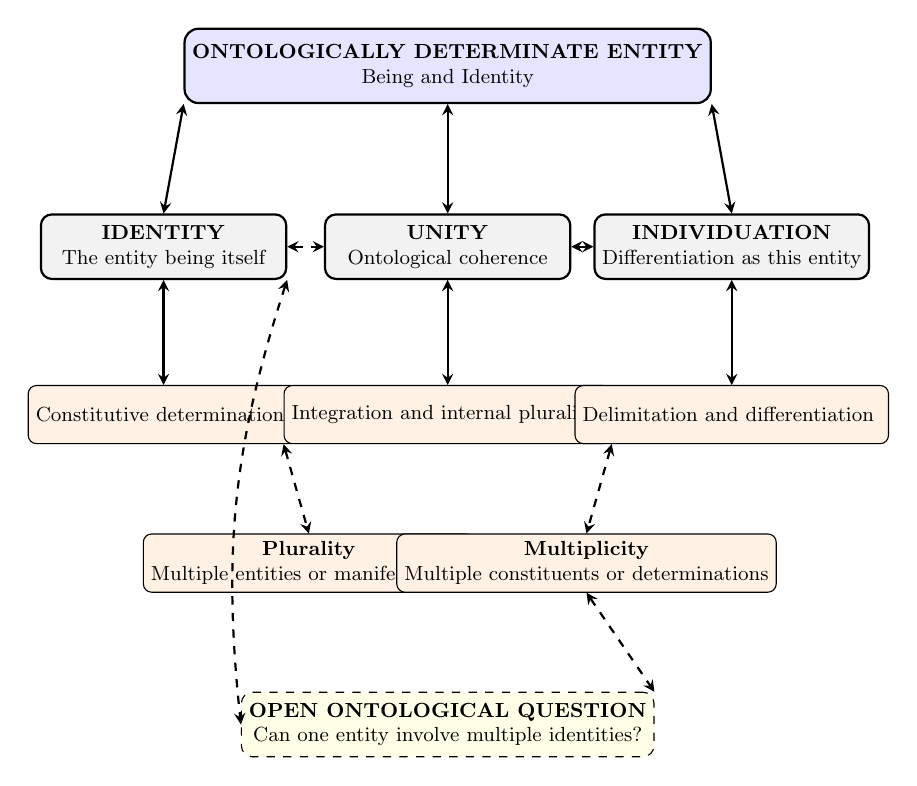
\begin{tikzpicture}[
        scale=0.82,
        transform shape,
        every node/.style={font=\small},
        core/.style={
            rectangle,
            rounded corners=5pt,
            draw=black,
            thick,
            minimum width=4.3cm,
            minimum height=1.15cm,
            align=center,
            fill=blue!10
        },
        concept/.style={
            rectangle,
            rounded corners=4pt,
            draw=black,
            thick,
            minimum width=3.8cm,
            minimum height=1cm,
            align=center,
            fill=gray!10
        },
        dimension/.style={
            rectangle,
            rounded corners=3pt,
            draw=black,
            minimum width=3.5cm,
            minimum height=0.9cm,
            align=center,
            fill=orange!10
        },
        openquestion/.style={
            rectangle,
            rounded corners=4pt,
            draw=black,
            dashed,
            minimum width=4.8cm,
            minimum height=1cm,
            align=center,
            fill=yellow!10
        },
        relation/.style={
            <->,
            thick,
            >=stealth
        },
        analytical/.style={
            <->,
            dashed,
            thick,
            >=stealth
        }
    ]

    % Central ontological entity
    \node[core] (entity) at (0,0) {
        \textbf{ONTOLOGICALLY DETERMINATE ENTITY}\\
        Being and Identity
    };

    % Three analytically distinct dimensions
    \node[concept] (identity) at (-4.4,-2.8) {
        \textbf{IDENTITY}\\
        The entity being itself
    };

    \node[concept] (unity) at (0,-2.8) {
        \textbf{UNITY}\\
        Ontological coherence
    };

    \node[concept] (individuation) at (4.4,-2.8) {
        \textbf{INDIVIDUATION}\\
        Differentiation as this entity
    };

    % Dimensions associated with each concept
    \node[dimension] (constitutive) at (-4.4,-5.4) {
        Constitutive determination
    };

    \node[dimension] (coherence) at (0,-5.4) {
        Integration and internal plurality
    };

    \node[dimension] (distinction) at (4.4,-5.4) {
        Delimitation and differentiation
    };

    % Plurality and multiplicity
    \node[dimension] (plurality) at (-2.15,-7.7) {
        \textbf{Plurality}\\
        Multiple entities or manifestations
    };

    \node[dimension] (multiplicity) at (2.15,-7.7) {
        \textbf{Multiplicity}\\
        Multiple constituents or determinations
    };

    % Open ontological question
    \node[openquestion] (question) at (0,-10.2) {
        \textbf{OPEN ONTOLOGICAL QUESTION}\\
        Can one entity involve multiple identities?
    };

    % Relations between the entity and its dimensions
    \draw[relation] (entity.south west) -- (identity.north);
    \draw[relation] (entity.south) -- (unity.north);
    \draw[relation] (entity.south east) -- (individuation.north);

    % Analytical distinctions
    \draw[analytical] (identity.east) -- (unity.west);
    \draw[analytical] (unity.east) -- (individuation.west);

    % Relations to associated dimensions
    \draw[relation] (identity.south) -- (constitutive.north);
    \draw[relation] (unity.south) -- (coherence.north);
    \draw[relation] (individuation.south) -- (distinction.north);

    % Internal plurality and multiplicity
    \draw[analytical] (coherence.south west) -- (plurality.north);
    \draw[analytical] (coherence.south east) -- (multiplicity.north);

    % The open question is not presented as a settled conclusion
    \draw[analytical] (identity.south east) to[bend right=12]
        (question.west);

    \draw[analytical] (multiplicity.south) -- (question.north east);

    \end{tikzpicture}

    \caption{The Relations Among Identity, Unity, and Individuation: Their Distinct Ontological Dimensions and the Open Question of Multiple Identities Within One Entity}
    \label{fig:identity-unity-and-individuation}
\end{figure}


The figure should be interpreted
as a conceptual representation rather
than as a causal, temporal, or hierarchical
sequence. It does not establish that
identity produces unity, that unity
produces individuation, or that
individuation is temporally subsequent
to identity.

It also preserves the open question
of whether one individual existent
may involve multiple identities.

\subsection{The Limits of an Ontology of Individuation}

The analysis establishes several
constraints for any subsequent
account of individuation.

First, individuation cannot be reduced
to identity, although the two are
ontologically related.

Second, individuation cannot be
identified with unity or with the
aggregation of components.

Third, distinction and qualitative
uniqueness do not provide sufficient
explanations of individuality.

Fourth, no universal principle of
individuation should be assumed
without establishing its applicability
to different kinds of existents.

Fifth, material, structural, and
relational conditions may contribute
to individuation, but their respective
roles must be examined rather than
presumed.

Sixth, individuation does not
automatically resolve the problem
of numerical identity and persistence.

Finally, the possibility of multiple
identities within one individual
existent remains open.

These constraints establish the
conceptual ground for a more precise
analysis of numerical identity and
the conditions under which an
individual remains the same existent.

\subsection{Concluding Formulation}

Individuation is the ontological
problem of how an existent is
constituted as a distinct individual
existent.

It is related to identity because
the individual is the existent whose
determinate character is under
consideration. It is related to unity
because an individual may constitute
a unity, including a unity involving
internal plurality. It is related to
distinction because individuation
concerns the constitution of an
existent as distinct.

Nevertheless, individuation cannot
be reduced to any of these concepts.

The central principle established
in this section is therefore:

\begin{quote}
Individuation concerns the ontological
constitution of an existent as an
individual. It is related to identity,
unity, and distinction, but cannot
be exhaustively explained through
any one of them.
\end{quote}

This principle establishes the basis
for examining numerical identity:
whether an individuated existent
remains one and the same existent
across different conditions and
transformations.
